\documentclass{beamer}
%\mode<presentation>
\usepackage[utf8]{inputenc}
\usepackage[english]{babel}
\usetheme{CambridgeUS}
\usecolortheme{dolphin}
\usepackage{amsmath,amssymb,amsfonts, bm}
\usepackage{mathpazo}
\usepackage{graphicx,tabularx,epsfig}
\usepackage{subcaption}
\usepackage{rotating}
\DeclareGraphicsExtensions{.pdf,.png,.jpg,.svg}


\title[Numerical hydrodynamics]{How does viscosity and the speed of sound effect spatial asymmetries in heavy ion collisions?}
\author{\underline{Attila Bagoly}, Máté Csanád}
\date[4 December, 2014]{14. ZIMÁNYI WINTER SCHOOL ON HEAVY ION PHYSICS\\ 4 December, 2014}
\institute[ELTE]{Eötvös University}
\begin{document}

\begin{frame}
  \titlepage
\end{frame}

\begin{frame}
\frametitle{Motivation}
\begin{itemize}
\item how some simple effects influence time evolution of asymmetries
\item  effects which can't be discussed analytically
\item not real initial condition (e.g. from Monte-Carlo simulation): real simulation mixes effects
\item initial condition close to exact solution but more realistic
\end{itemize}
\end{frame}

\begin{frame}
\frametitle{Contents}
\tableofcontents
\end{frame}

\section{Equations of hydrodynamics}
\begin{frame}
\frametitle{Equations of hydrodynamics}
\begin{itemize}
\item Nonrelativistic hydrodynamics:
\begin{equation}
\frac{\partial \rho}{\partial t} + \bm{\nabla}\rho\bm{v}=0
\end{equation}
\begin{equation}
\rho\Big(\frac{\partial \bm{v}}{\partial t}+(\bm{v\nabla})\bm{v}\Big)=-\bm{\nabla}p +\mu\Delta\bm{v}+\Big(\zeta+\frac{\mu}{3}\Big)\bm{\nabla}(\bm{\nabla v})+\bm{f}
\end{equation}
\begin{equation}
\frac{\partial \varepsilon}{\partial t}+\bm{\nabla}\varepsilon\bm{v}=-p\bm{\nabla v}+\bm{\nabla(\sigma v)}
\end{equation}

\item We need an EoS:
\begin{equation}
\varepsilon=\kappa(T)p
\end{equation}

\item Relativistic case:
\begin{large}
\begin{equation}
T^{\mu\nu}=\big(\varepsilon+p\big)\frac{u^\mu u^\nu}{c^2}-pg^{\mu\nu},\quad \partial_\mu T^{\mu\nu}=0
\end{equation}
\end{large}
\end{itemize}
\end{frame}

%\section{Multipole solution}
%\begin{frame}
%\frametitle{Multipole solution}
%\begin{itemize}
%\item New exact solution of relativistic hydrodynamics by Máté Csanád and András Szabó, published Phys.Rev. C90 (2014) 054911
%\item The solution
%\begin{equation}
%u^\mu=\gamma\Big(1, \frac{\dot{R}}{R}r\cos\varphi, \frac{\dot{R}}{R}r\sin\varphi,\frac{\dot{R}}{R}z\Big)
%\end{equation}
%\begin{equation}
%n=n_0\Big(\frac{\gamma R_0}{R}\Big)^3\nu(s)
%\end{equation}
%\begin{equation}
%p=p_0\Big(\frac{\gamma R_0}{R}\Big)^{3+\frac{3}{\kappa}}
%\end{equation}
%\item Where $\gamma=\frac{1}{\sqrt{1-(r^2+z^2)\dot{R}^2/R^2}}$
%\item That's a solution if $R=R_0t$
%\item The s scale variable with any asymmetries 
%\begin{equation}
%s=\frac{r^2}{R^2}\Big(1+\varepsilon_{N}\cos N\varphi\Big)+\frac{z^2}{R^2}
%\end{equation}
%\end{itemize}
%\end{frame}
%$u^\mu=\gamma\Big(1, \frac{\dot{R}}{R}r\cos\varphi, \frac{\dot{R}}{R}r\sin\varphi,\frac{\dot{R}}{R}z\Big)$
%$n=n_0\Big(\frac{\gamma R_0}{R}\Big)^3\nu(s)$, $p=p_0\Big(\frac{\gamma R_0}{R}\Big)^{3+\frac{3}{\kappa}}$
%\item Where $\gamma=\frac{1}{\sqrt{1-(r^2+z^2)\dot{R}^2/R^2}}$
%\item That's a solution if $R=R_0t$
%\item The s scale variable with any asymmetries 
%$s=\frac{r^2}{R^2}\Big(1+\varepsilon_{N}\cos N\phi\Big)+\frac{z^2}{R^2}$

\begin{frame}
\frametitle{Multipole solution}
  \begin{minipage}{0.39\textwidth}
    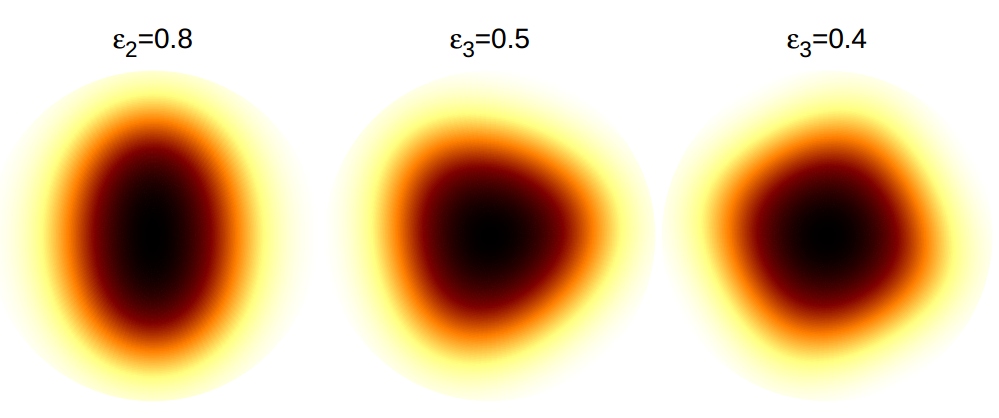
\includegraphics[scale=0.16]{pic/a1}

    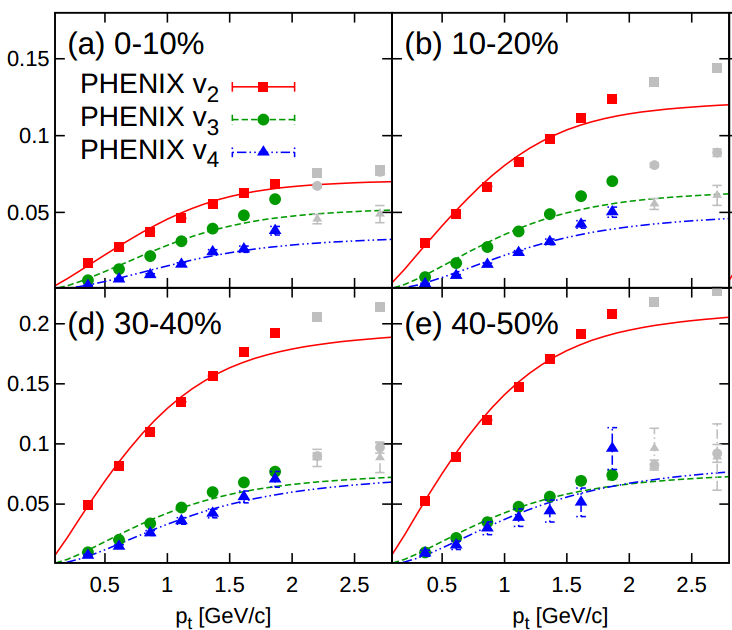
\includegraphics[scale=0.2]{pic/a2}
  \end{minipage}
  \begin{minipage}{0.60\textwidth}
  \begin{itemize}
\item New exact solution of relativistic hydrodynamics by Máté Csanád and András Szabó, published Phys.Rev. C90 (2014) 054911
\item The solution in cylindrical coordinates:
$u^\mu=\frac{x^\mu}{\tau}$, $n=n_f\big(\frac{\tau_f}{\tau}\big)^3\nu(s)$, $p=p_f\big(\frac{\tau_f}{\tau}\big)^{3+3/\kappa}$
\item Where $\tau$ is the coordinate-proper time, $\tau_f$ is the freeze-out proper time
\item The s scale variable with any asymmetries 
$s=\frac{r^N}{R^N}\Big(1+\epsilon_{N}\cos N\phi\Big)+\frac{z^N}{R^N}$
\item That's a solution if $R=u_tt$
\end{itemize}
  \end{minipage}
\end{frame}


\section{Numerical scheme}
\begin{frame}
\frametitle{Numerical scheme}
\begin{itemize}
\item At mid-rapidity distributions have local maximum and are constant in its environment, so enough to solve hydro in 2+1 dimension
\item Transform equations to advection from: $\partial_t Q_i+\partial_x F_i(Q)+\partial_y G_i(Q)=0$
\item Solve numerically: discretization
\item Finite volume method: average of quantities in control volume, that contains the grid point
\item Problem: we have to evaluate fluxes between grid points, exactly not possible 
\item Instability: we can add to real solution a wave solution which is null at grid points $\rightarrow$ Courant–Friedrichs–Lewy condition (e.g. $C=u\Delta t/ \Delta x < 1$)
\item 2 spatial dimension difficult $\rightarrow$ operator splitting
\item Viscosity: ideal substep + step only with viscous fluxes
\end{itemize}
\end{frame}

\begin{frame}
\frametitle{Numerical scheme: MUSTA method}
\begin{itemize}
\item This method was published by E. F. Toro et al, 2006, J. Comp. Phys
\item The $l^{\rm th}$ predicted values: $Q^{(l)}_{i/(i+1)}$, $F^{(l)}_{i/(i+1)}\equiv F\big(Q^{(l)}_{i/(i+1)}\big)$
\item Initially: $Q^{(0)}_i\equiv Q^n_i$,  $Q^{(0)}_{i+1}\equiv Q^{n}_{i+1}$
\item Intermediate value and flux:
\end{itemize}
\begin{equation}
Q^{(l)}_{i+\frac{1}{2}}=\frac{1}{2}\Big[Q^{(l)}_i+Q^{(l)}_{i+1}\Big]-\frac{1}{2}\frac{\Delta t}{\Delta x}\Big[F^{(l)}_{i+1}-F^{(l)}_i\Big], \quad F_M^{(l)} \equiv F\big(Q^{(l)}_{i+\frac{1}{2}}\big)
\end{equation}


\begin{itemize}
\item Corrected flux:
\end{itemize}
\begin{equation}
F^{(l)}_{i+\frac{1}{2}}=\frac{1}{4}\Big[F^{(l)}_{i+1}+2F^{(l)}_M+F^{(l)}_{i}-\frac{\Delta x}{\Delta t}\Big(Q^{(l)}_{i+1}-Q^{(l)}_i\Big)\Big]
\end{equation}
\begin{itemize}
\item Next prediction to compute corrected flux:
\end{itemize}
\begin{equation}
Q_i^{(l+1)}=Q^{(l)}_i-\frac{\Delta t}{\Delta x}\Big[F^{(l)}_{i+\frac{1}{2}}-F^{(l)}_i\Big]
\end{equation}
\begin{equation}
Q_{i+1}^{(l+1)}=Q^{(l)}_{i+1}-\frac{\Delta t}{\Delta x}\Big[F^{(l)}_{i+1}-F^{(l)}_{i+\frac{1}{2}}\Big]
\end{equation}
\end{frame}

\section{Code testing}
\begin{frame}
\frametitle{Code testing}
\begin{itemize}
\item We tested our code with exact solutions (from PRC67 (2003)):
$s=\frac{x^2}{X^2(t)}+\frac{y^2}{Y^2(t)}$, $\rho = \rho_0\frac{V_0}{V}e^{-s}$,  $p=p_0\big(\frac{V_0}{V}\big)^{1+\frac{1}{\kappa}}$, $\bm{v}(t, \bm{r})=\big(\frac{\dot{X}}{X}x, \frac{\dot{Y}}{Y}y\big)$, $\ddot{X}X=\ddot{Y}Y=\frac{T_i}{m}\big(\frac{V_0}{V}\big)^{\frac{1}{\kappa}}$, $V=X(t)Y(t)$
\item Relative difference between exact and numerical solution ($X=Y$ and $X\neq Y$ case):
\end{itemize}
\begin{center}
\begin{figure}[H]
	\centering
    \begin{subfigure}[b]{0.49\textwidth}
    		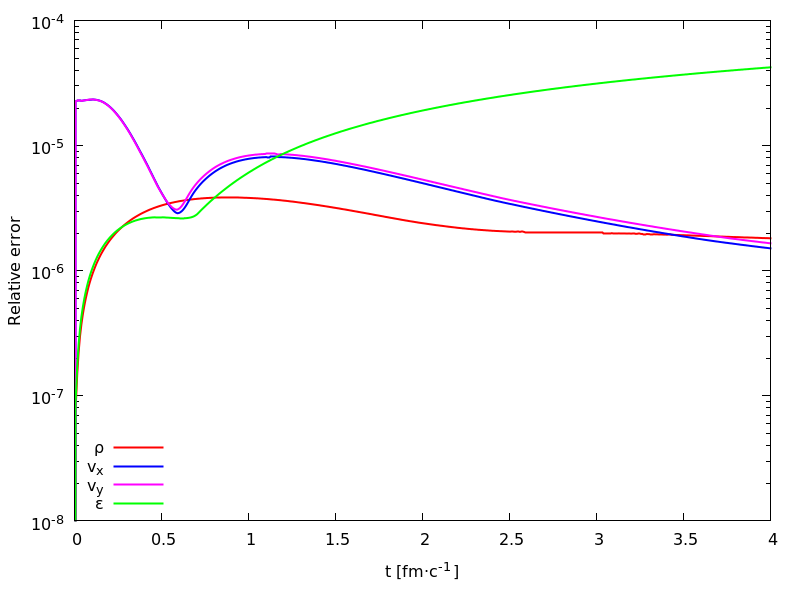
\includegraphics[width=\textwidth]{pic/sym}
	\end{subfigure}
	\begin{subfigure}[b]{0.49\textwidth}
        	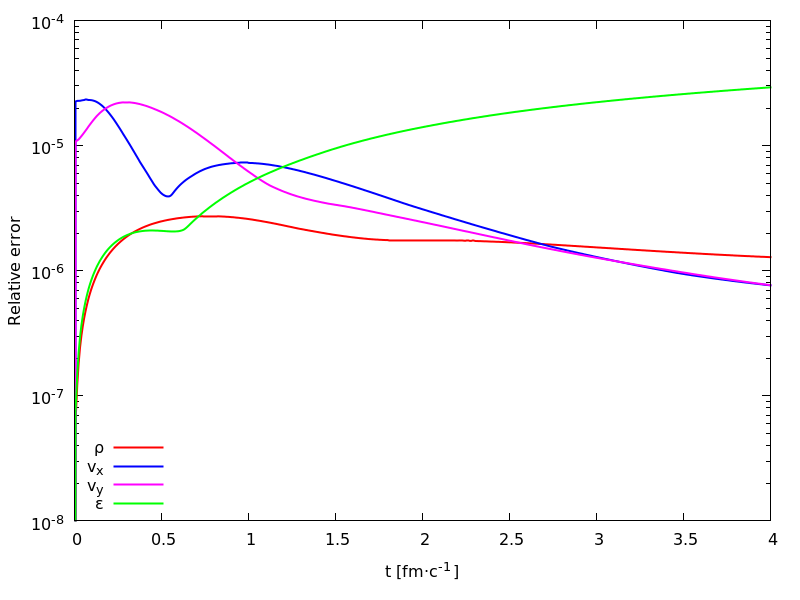
\includegraphics[width=\textwidth]{pic/asym}
	\end{subfigure}
\end{figure}
\end{center}
\end{frame}

\section{}
\begin{frame}
\frametitle{Description of asymmetries}
\begin{itemize}
\item We defined as asymmetry parameters: $\varepsilon_n=\langle \cos(n\phi)\rangle_{\rho/w/p}$
\item The $w=\exp{(-v_x^2-v_y^2)}$ is defined to calculate the asymmetry of speed distribution
\item This $\varepsilon_n$ not equal with the $\epsilon$ in $s$ scale variable ($\rho,\,p \propto \exp{(-s)}$)
\item Initially we can approximate $\varepsilon_n$ with $\epsilon_n$ using Taylor-series:
\begin{equation}
\varepsilon_1=\frac{(\epsilon_2+\epsilon_4)\epsilon_3}{2+\sum_{n=2}^4\epsilon_n^2}
\end{equation}
\begin{equation}
\varepsilon_2=\frac{-\epsilon_2+\epsilon_2\epsilon_4}{2+\sum_{n=2}^4\epsilon_n^2}
\end{equation}
\begin{equation}
\varepsilon_3=\frac{-\epsilon_3}{2+\sum_{n=2}^4\epsilon_n^2}
\end{equation}
\begin{equation}
\varepsilon_4=\frac{-\epsilon_4+\frac{1}{2}\epsilon_2^2}{2+\sum_{n=2}^4\epsilon_n^2}
\end{equation}
\end{itemize}
\end{frame}

\section{Nonrelativistic results}

\begin{frame}
\frametitle{Effect of viscosity}
\begin{center}
\begin{itemize}
\item In energy and mass density the viscosity makes slower the disappearance 
\item In speed distribution makes faster
\end{itemize}
\begin{figure}[H]
	\centering
    \begin{subfigure}[b]{0.49\textwidth}
    		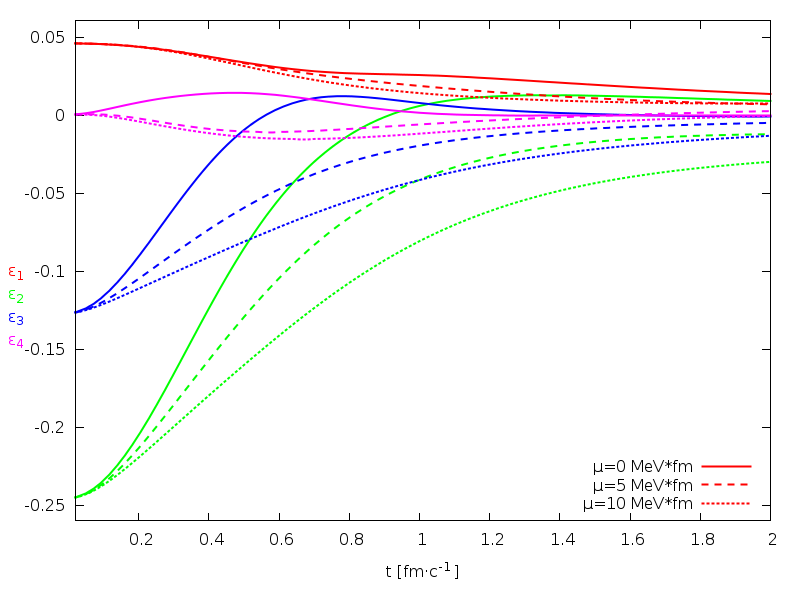
\includegraphics[width=\textwidth]{pic/res/nonrel/eps_visc_r}
	\end{subfigure}
	\begin{subfigure}[b]{0.49\textwidth}
        	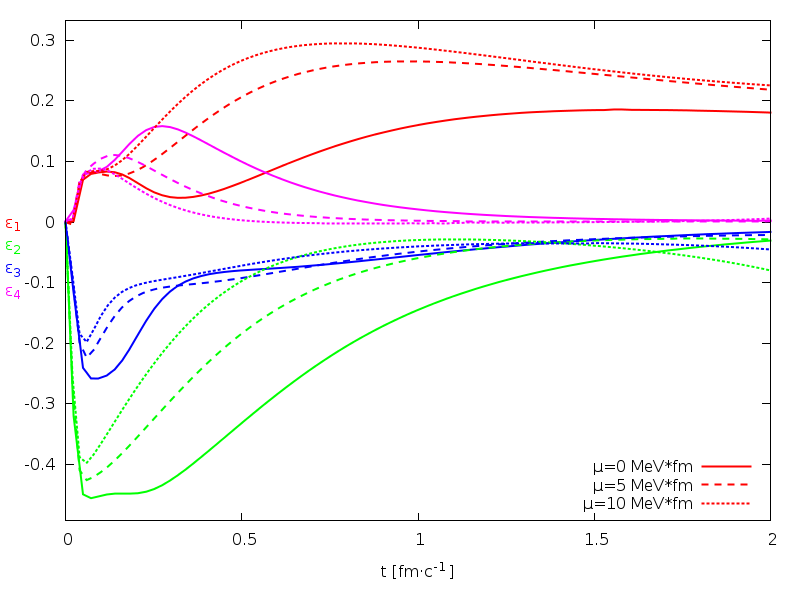
\includegraphics[width=\textwidth]{pic/res/nonrel/eps_visc_v}
	\end{subfigure}
\end{figure}
\end{center}
\end{frame}

\begin{frame}
\frametitle{Effect of viscosity: The time evolution of energy density}
\begin{minipage}{0.04\textwidth}
\rotatebox[origin=c]{90}{$\qquad$\scalebox{0.85}{$\mu=0\;\textnormal{MeVfm/c}$}}
\rotatebox[origin=c]{90}{\scalebox{0.85}{$\mu=10\;\textnormal{MeVfm/c}$}}
\end{minipage}
\begin{minipage}{0.95\textwidth}
\begin{center}
    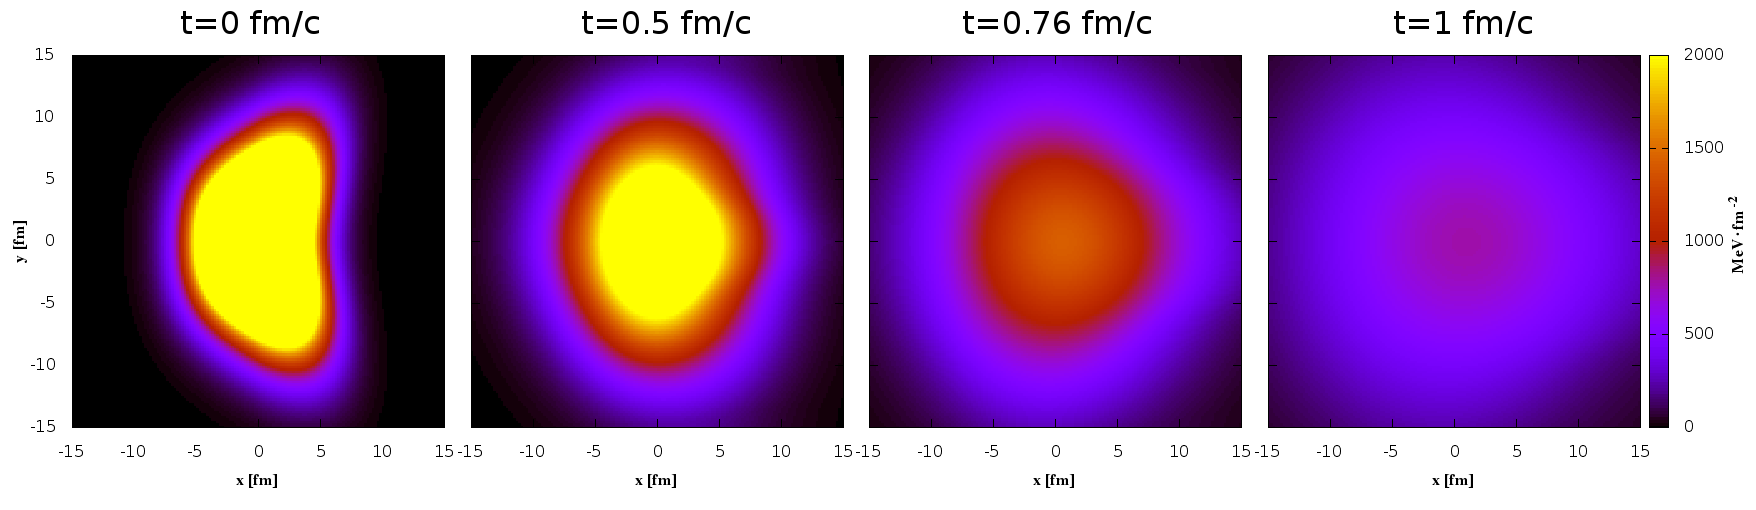
\includegraphics[scale=0.19]{pic/res/nonrel/anim/ev0}

    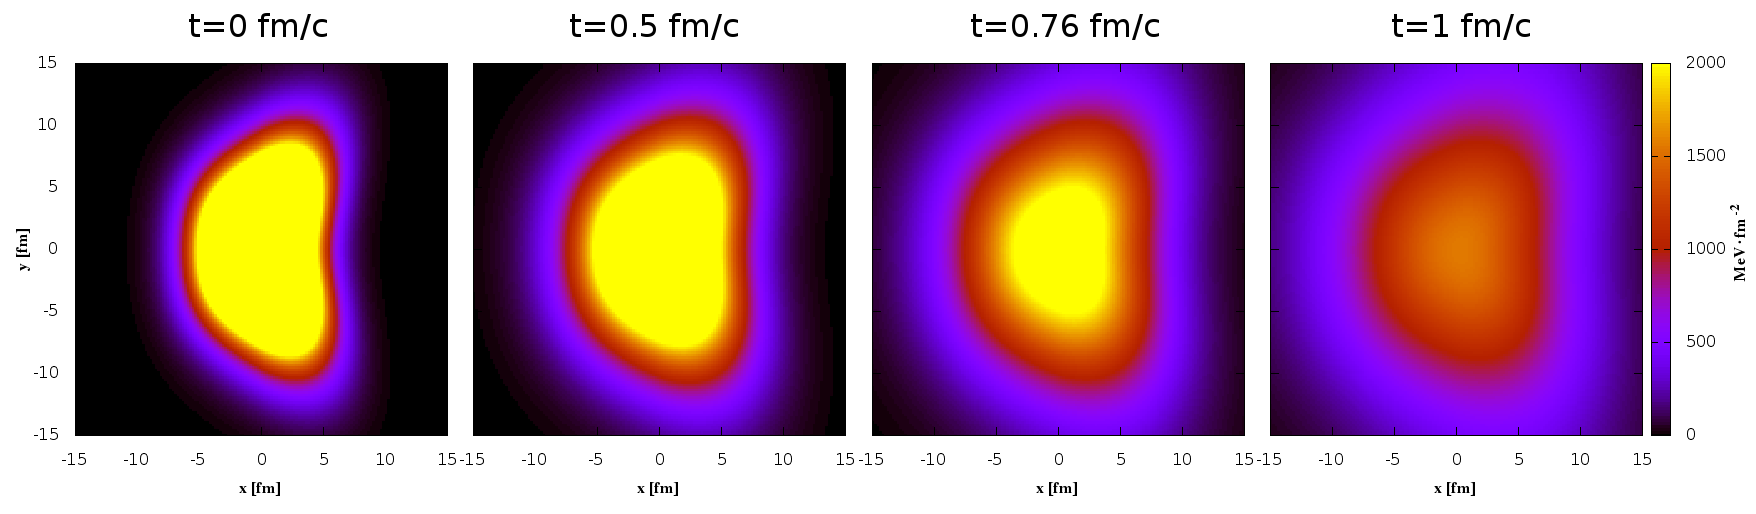
\includegraphics[scale=0.19]{pic/res/nonrel/anim/ev10}
\end{center}
\end{minipage}
\end{frame}
\begin{frame}
\frametitle{Effect of viscosity:  The time evolution of speed distribution}
\begin{minipage}{0.04\textwidth}
\rotatebox[origin=c]{90}{$\qquad$\scalebox{0.85}{$\mu=0\;\textnormal{MeVfm/c}$}}
\rotatebox[origin=c]{90}{\scalebox{0.85}{$\mu=10\;\textnormal{MeVfm/c}$}}
\end{minipage}
\begin{minipage}{0.95\textwidth}
\begin{center}
    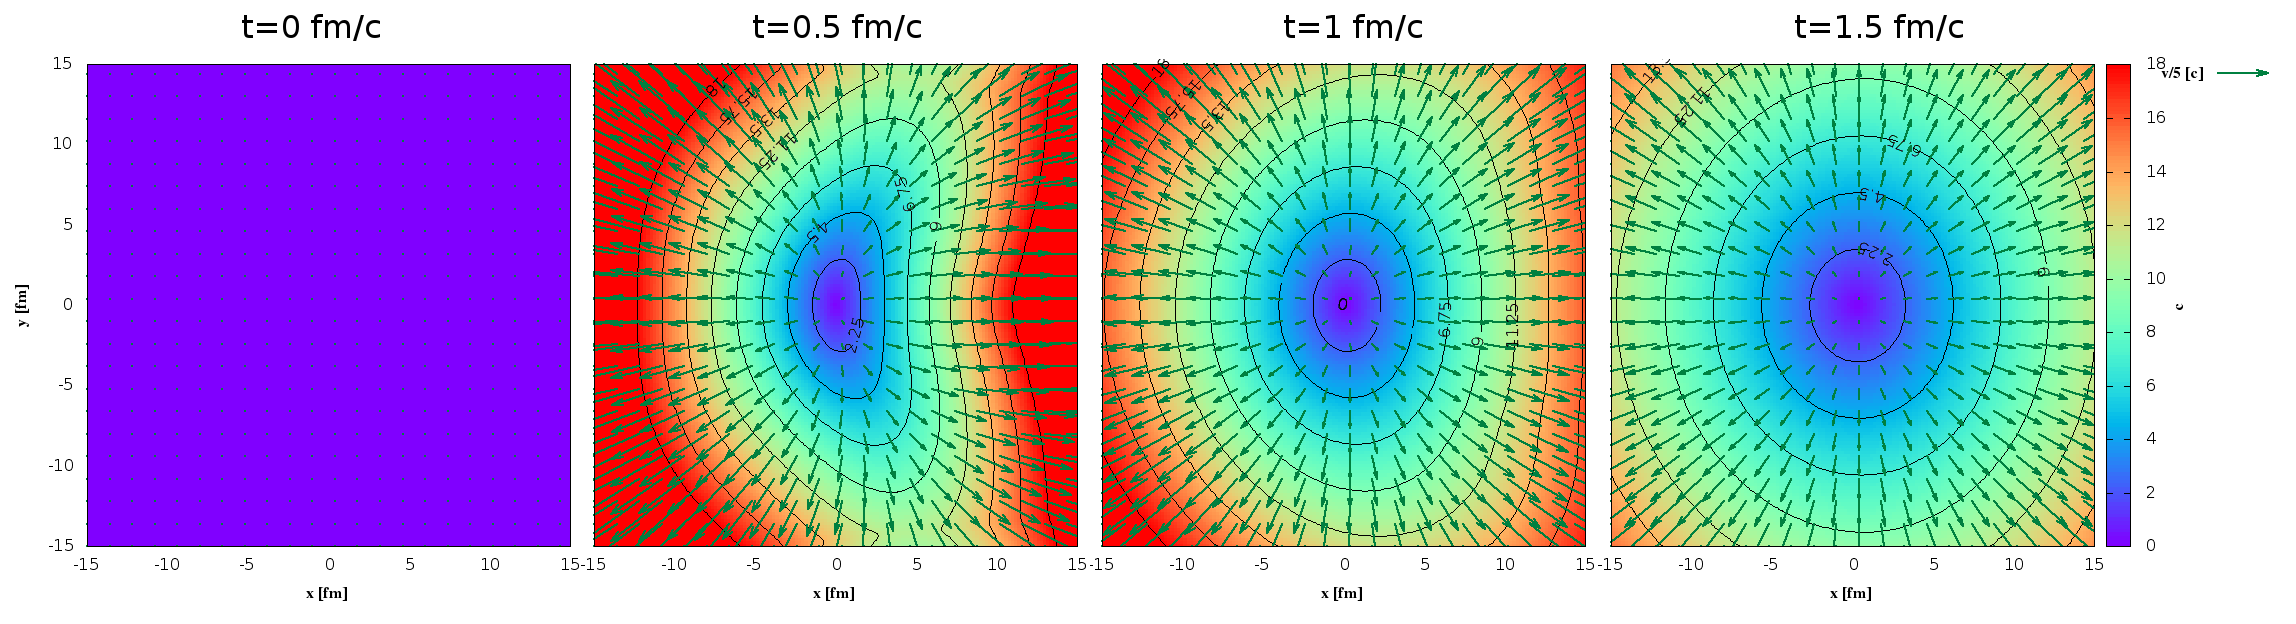
\includegraphics[scale=0.15]{pic/res/nonrel/anim/vv0}

    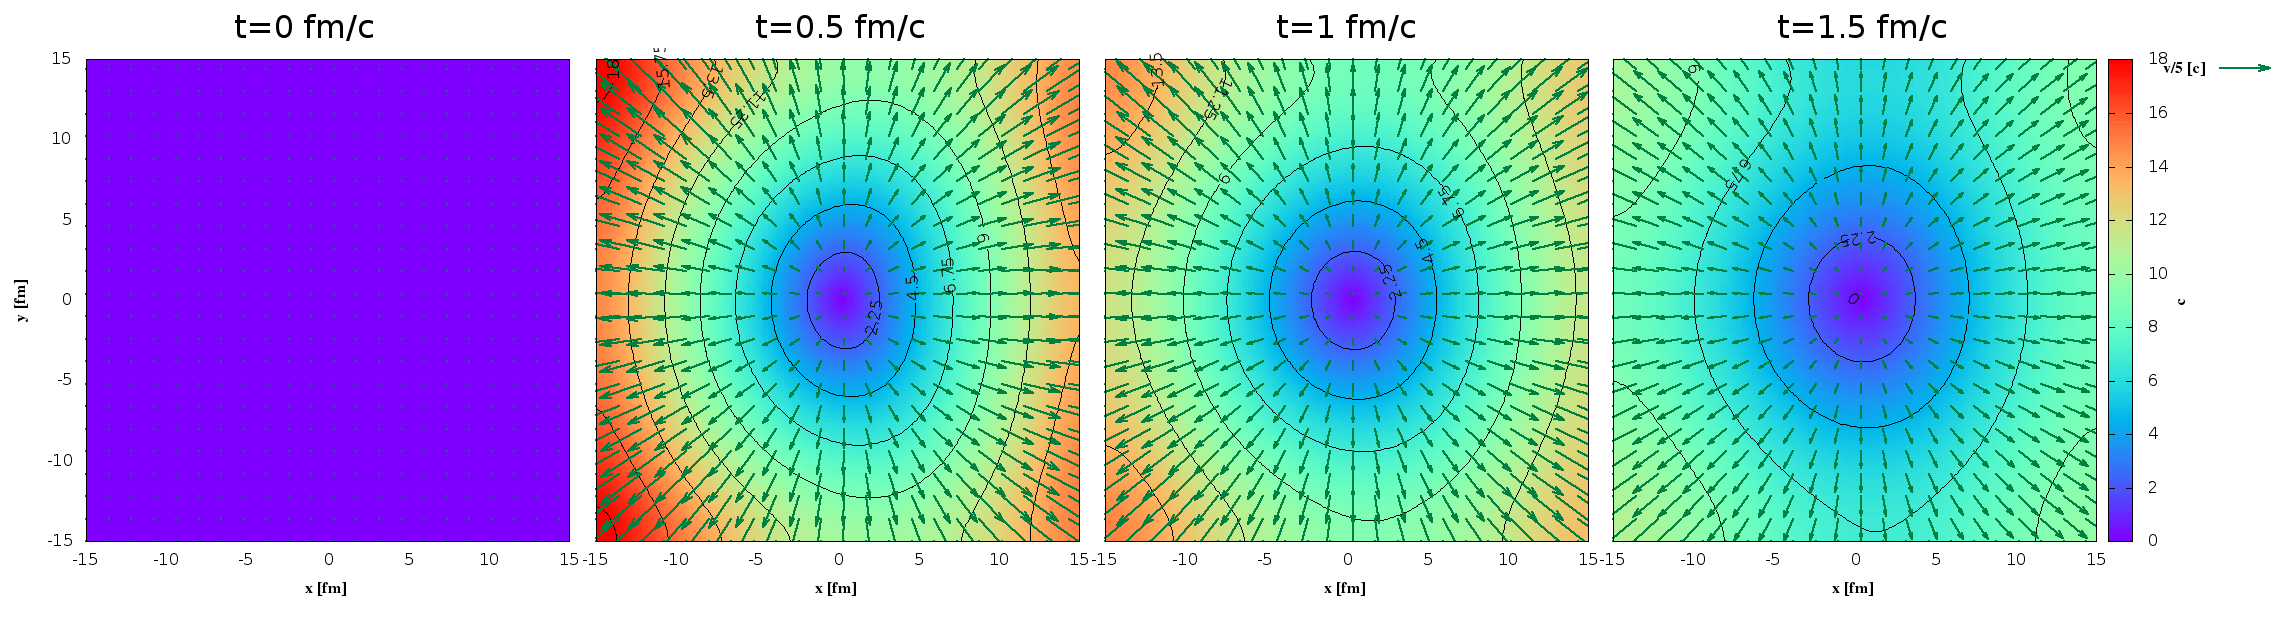
\includegraphics[scale=0.15]{pic/res/nonrel/anim/vv10}
\end{center}
\end{minipage}
\end{frame}

\begin{frame}
\frametitle{Effect of speed of sound}
\begin{center}
\begin{itemize}
\item As we expected the reduction of speed of sound makes the time evolution of asymmetries slower
\end{itemize}
\begin{figure}[H]
	\centering
    \begin{subfigure}[b]{0.49\textwidth}
    		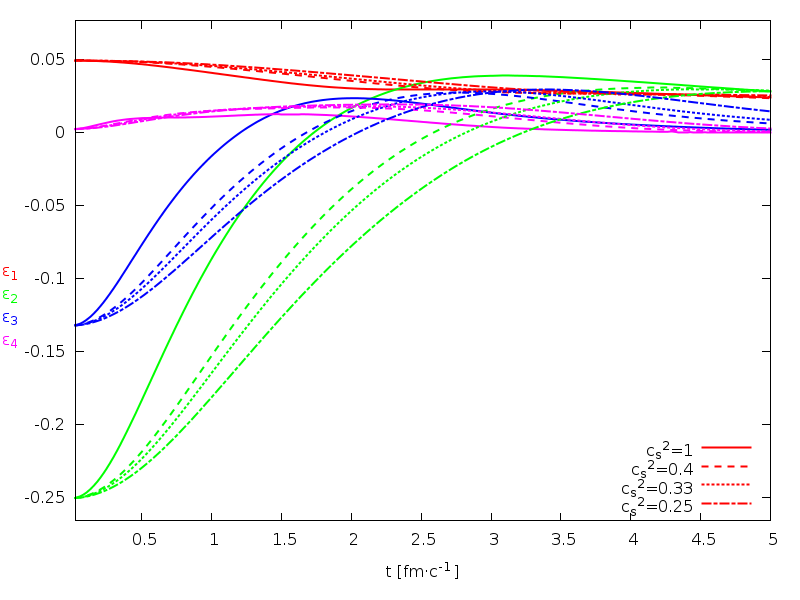
\includegraphics[width=\textwidth]{pic/res/nonrel/eps_cs2_r}
	\end{subfigure}
	\begin{subfigure}[b]{0.49\textwidth}
        	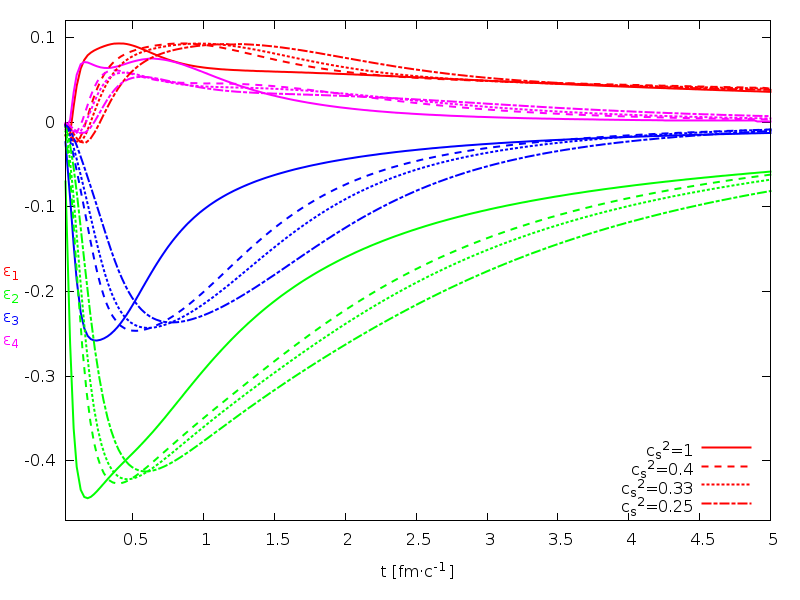
\includegraphics[width=\textwidth]{pic/res/nonrel/eps_cs2_v}
	\end{subfigure}
\end{figure}
\end{center}
\end{frame}

\begin{frame}
\frametitle{Effect of pressure gradient}
\begin{center}
\begin{itemize}
\item The increase gradient of pressure makes the flow faster, so the asymmetries disappear faster
\end{itemize}
\begin{figure}[H]
	\centering
    \begin{subfigure}[b]{0.49\textwidth}
    		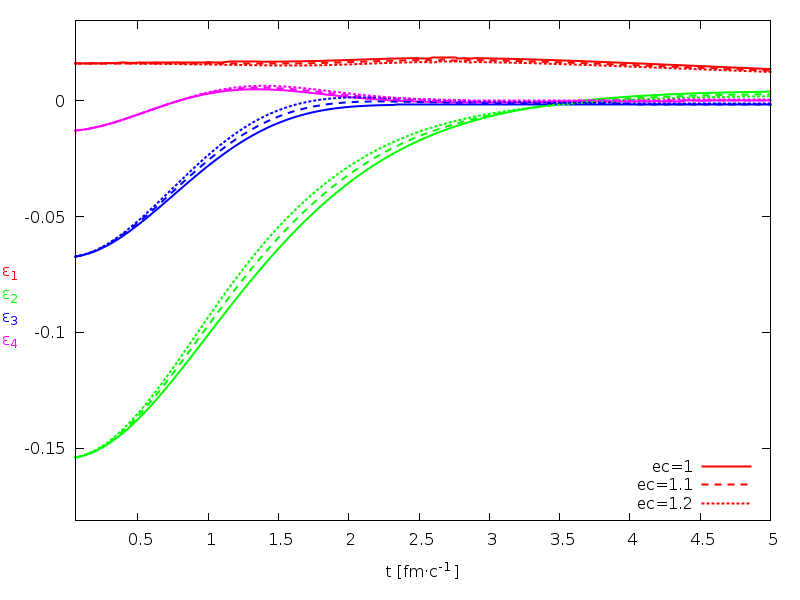
\includegraphics[width=\textwidth]{pic/res/nonrel/eps_ec_r}
	\end{subfigure}
	\begin{subfigure}[b]{0.49\textwidth}
        	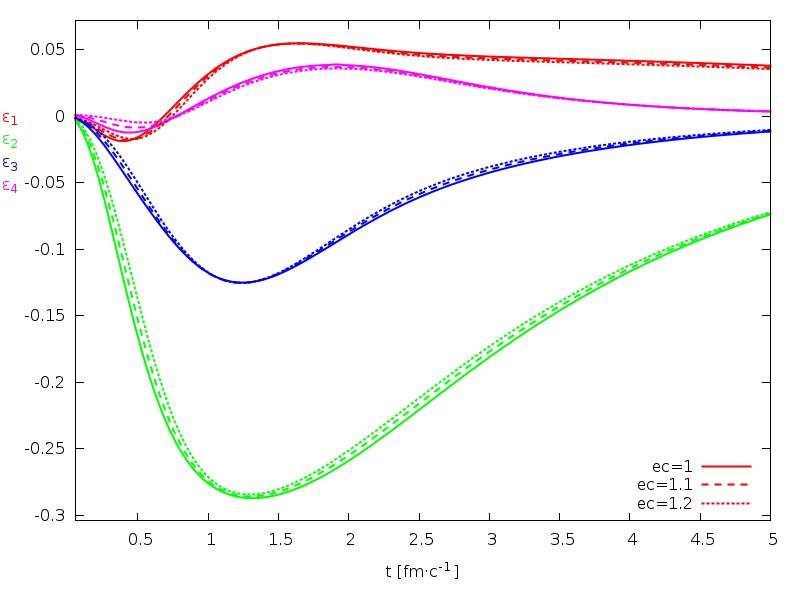
\includegraphics[width=\textwidth]{pic/res/nonrel/eps_ec_v}
	\end{subfigure}
\end{figure}
\end{center}
\end{frame}

\section{Relativistic results}
\begin{frame}
\frametitle{Effect of speed of sound}
\begin{center}
\begin{itemize}
\item Same as nonrelativistic case
\item Different time to hadronization
\end{itemize}
\begin{figure}[H]
	\centering
    \begin{subfigure}[b]{0.49\textwidth}
    		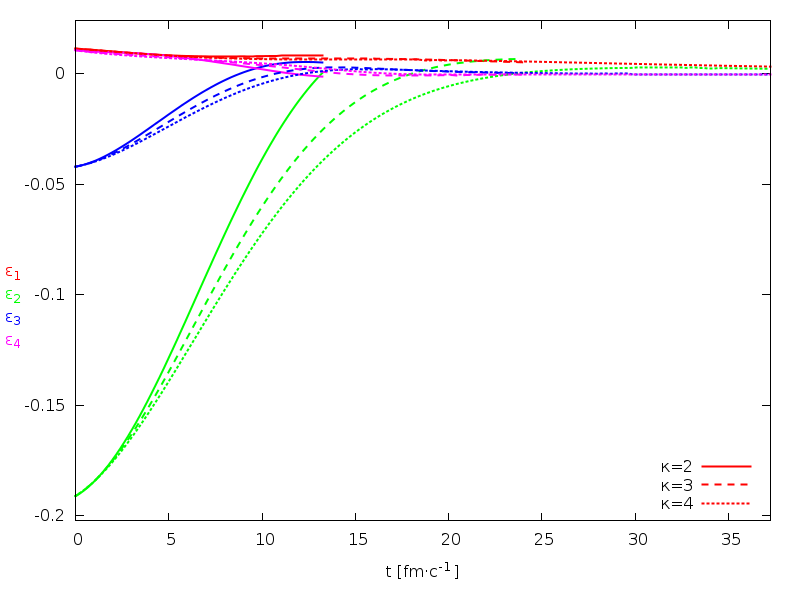
\includegraphics[width=\textwidth]{pic/res/rel/eps_kappa_n}
	\end{subfigure}
	\begin{subfigure}[b]{0.49\textwidth}
        	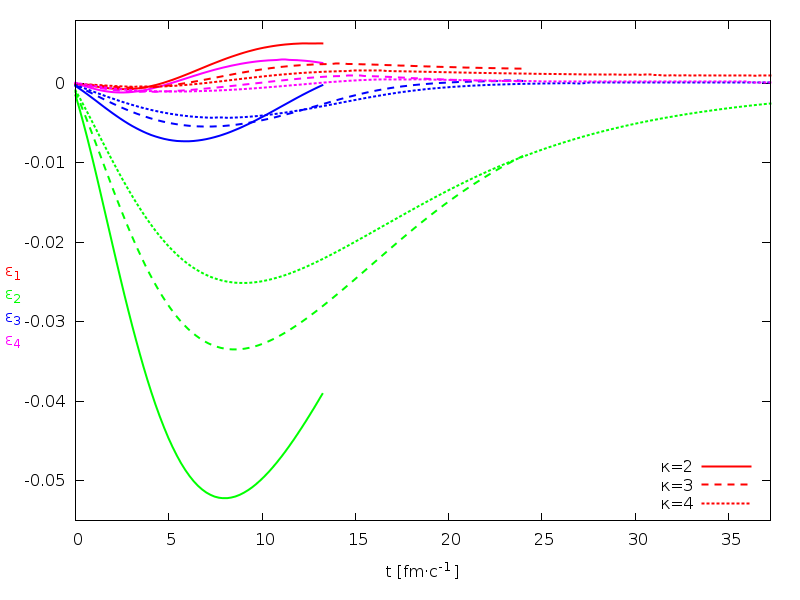
\includegraphics[width=\textwidth]{pic/res/rel/eps_kappa_v}
	\end{subfigure}
\end{figure}
\end{center}
\end{frame}

\begin{frame}
\frametitle{Effect of pressure gradient}
\begin{center}
\begin{itemize}
\item Same as nonrelativistic case
\end{itemize}
\begin{figure}[H]
	\centering
    \begin{subfigure}[b]{0.49\textwidth}
    		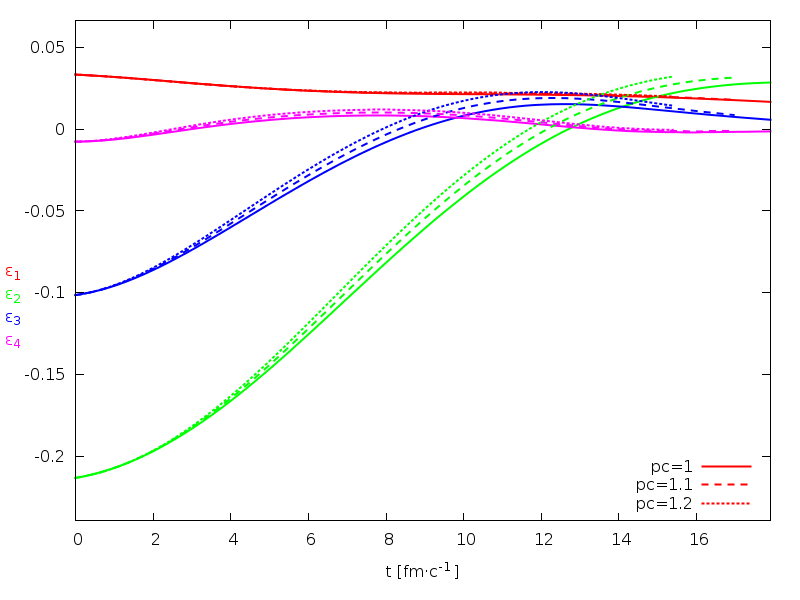
\includegraphics[width=\textwidth]{pic/res/rel/eps_pc_n}
	\end{subfigure}
	\begin{subfigure}[b]{0.49\textwidth}
        	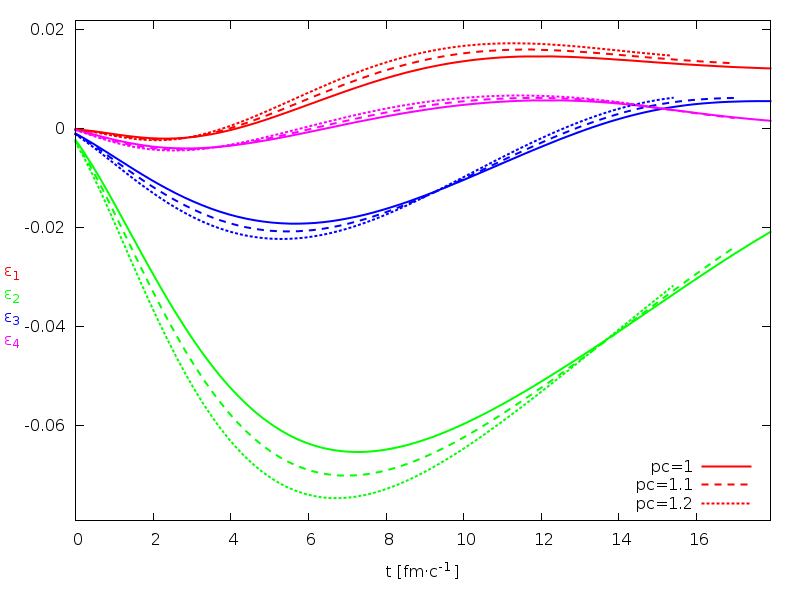
\includegraphics[width=\textwidth]{pic/res/rel/eps_pc_v}
	\end{subfigure}
\end{figure}
\end{center}
\end{frame}

\section{Hadronization}
\begin{frame}
\frametitle{Hadronization}
\begin{itemize}
\item Maxwell-Jüttner type source function: 
$S(x, p)d^4x=\mathcal{N}n(x)\exp{\bigg(-\frac{p_\mu u^\mu}{T(x)}\bigg)}H(\tau)p_\mu d^3\frac{u_\mu d^3x}{u^0} d\tau$
\item With source function we can simply calculate the measurable quantities:
$v_n(p_t)=\langle\cos(n\varphi)\rangle_{N}=\frac{1}{N(p_t)}\int_0^{2\pi} N(p_t, \varphi)\cos(n\varphi)d\varphi$
\end{itemize}
\begin{center}
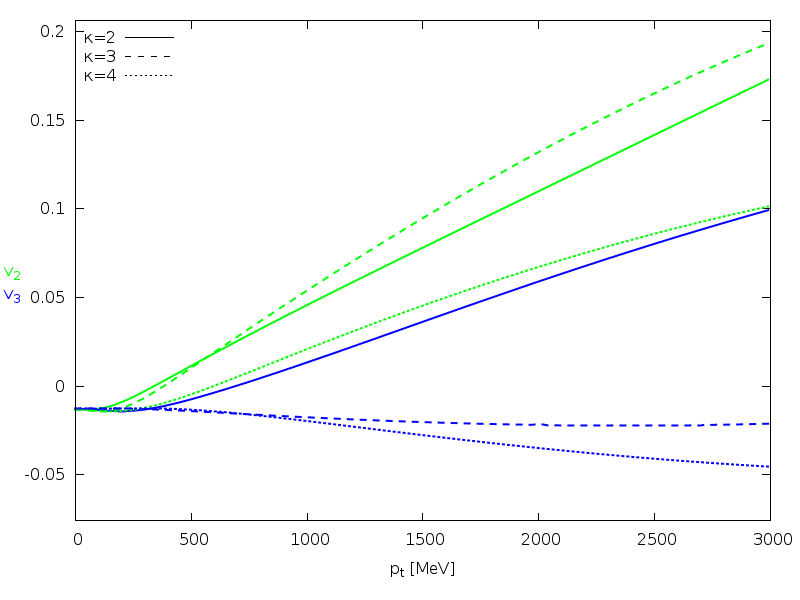
\includegraphics[scale=0.24]{pic/res/rel/vn_kappa}
\end{center}
\end{frame}

\section{Summary}
\begin{frame}
\frametitle{Summary}
\begin{itemize}
%\item New multipole solution published Phys.Rev. C90 (2014) 054911
%\item Numerical method for solving hydro equations
%\item Nonrelativistic case: how viscosity, speed of sound and gradient of pressure effect on spatial asymmetry
%\item Relativistic case: how speed of sound and gradient of pressure effect on spatial asymmetry
%\item Measurable quantities
\item Motivation: how some simple effects affect time evolution of asymmetries
\item No much chance for analytic discussion so we used numerical methods
\item Initial condition was very close to the existing exact solutions, but more realistic
\item Viscosity makes slower the disappearance of asymmetries in energy density and faster in speed distribution
\item Smaller speed of sound makes slower time evolution in all distribution, more time to hadronization
\end{itemize}
\end{frame}

\end{document}

